Filet à l'anglaise est une méthode de cuisson française pour un filet de poisson ou de volailles, qui consiste à le faire poêler d'abord dans une grande quantité d'huile chaude, puis à le passer rapidement au four pour le finir en rôtissage. Le terme 'à l'anglaise' signifie que la viande est cuite au four, ce qui a peut-être été adopté de la manière anglaise traditionnelle de cuire des viandes.

Par exemple, pour cuire des sardines, nous pouvons  utiliser plusieurs méthodes de cuisson. Par exemple, on peut les faire griller à la broche, les faire poêler dans une sauteuse ou les mettre à four. Pour le cas de la broche, il est nécessaire de passer les sardines au four préalablement pour les égoutter. Avec la méthode à la poêle, vous pouvez choisir d'utiliser de l'huile ou du beurre et ajouter des épices selon votre goût. Enfin, dans le cas d'une cuisson au four, vous pouvez les mettre dans une papillote avec un peu d'huile et d'épices pour enrichir le goût. Chaque méthode de cuisson apporte son côté unique à ces petits poissons, il reste donc à vous de choisir la méthode qui vous convient le mieux !


\begin{figure}[h!]
    \centering
    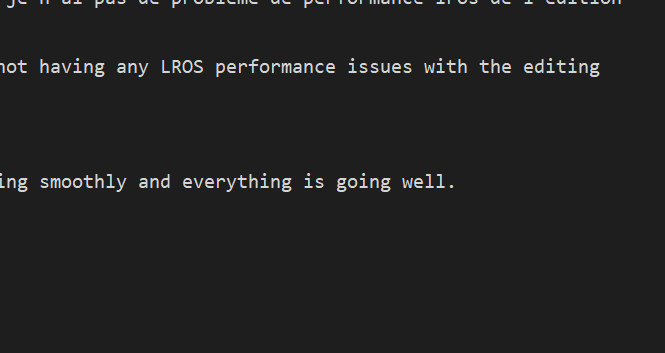
\includegraphics[width=0.8\textwidth]{figures/default/default/default/fig1.png}
    \caption{Caption here}
    \label{fig:default_default_1}
\end{figure}




